\Chapter{Tesztelés}


\Section{Jquerry test}


A program megvalósításához szóba jött a Jquerry használata is, és ezáltal az is, hogy vajon a Jquerry-s vagy a sima context-re rajzolás lehet-e a gyorsabb.

Ehhez a vizsgálathoz két példa program is készült, az egyik azt vizsgálta, hogy melyik megoldás milyen gyorsasággal rajzol ki. 

1000-től 29000-ig vizsgáltuk a kirajzolást ezresével növelve a méretet, ugyanazzal a kitöltéssel, mérettel, és már itt láttuk, hogy a Jquerry sokkal lassabb. Az itt kapott futási időket \Aref{fig:pieces}. grafikon tartalmazza. 

\begin{figure}[h]
	\centering
	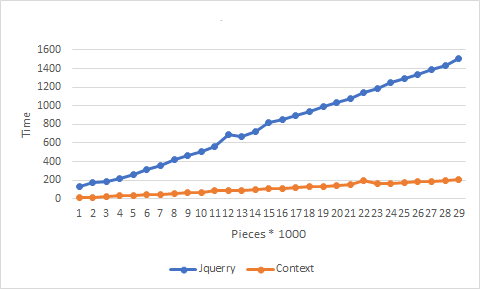
\includegraphics[scale=1]{images/pieces.png}
	\caption{Jquerry vs context kirajzolás daraszám alapján.}
	\label{fig:pieces}
\end{figure}


De vizsgáltunk egy másik szempontot is, még pedig, hogy ha a körök méretét növeljük, akkor melyik a gyorsabb. 

10-től 290-es méretig rajzoltattunk ki köröket tizesével növelve a méretet, és itt is láthattuk, hogy a Jquerry lassabb, így a programban azt a megoldást nem használtuk. Az itt kapott futási időket pedig \Aref{fig:radius}. grafikon tartalmazza

\begin{figure}[h]
	\centering
	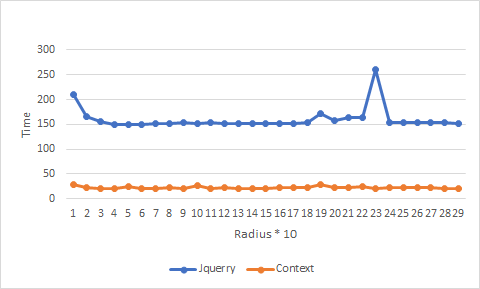
\includegraphics[scale=1]{images/radius.png}
	\caption{Jquerry vs context kirajzolás méret alapján.}
	\label{fig:radius}
\end{figure}

\Section{Program használata}

A program használata nagyon egyszerű, ha betöltött az oldal megjelennek a kis körök/részecskék. Azokon kívül alól az előző fejeztben \Aref{fig:html} már bemutatott, dolgokat láthatjuk. 

\textbf{Csúszkák}

 A csúszkák segítségével a részecskékre ható erőket lehet módosítani.


\textbf{Gombok}

A programban 2 gomb van ezek a pohár hozzáadás, illetve eltávolítás. A pohár hozzáadása gombbal egy poharat lehet a programhoz hozzáadni, az eltávolítóval meg nyilván eltávolítani. 

\textbf{Koordináták}

A pohár koordinátáit lehet még módosítani a programban. Amik már szintén az előző fejezetben \Aref{fig:pohar} bemutatott módon hatnak a pohárra. 

\textbf{Követelmények}

A programnak nincs szüksége semmi másra csak egy webböngészőre. Ami a mai világban már szinte mindenre elérhető. 

